\documentclass[11pt,a4paper]{article}

%====================== PACKAGES ======================
\usepackage[utf8]{inputenc}
\usepackage[T1]{fontenc}
\usepackage[margin=2.4cm]{geometry}
\usepackage{amsmath,amssymb,amsthm,mathtools}
\usepackage{booktabs}
\usepackage{array}
\usepackage{enumitem}
\usepackage{graphicx}
\usepackage{xcolor}
\usepackage[most]{tcolorbox}
\usepackage{pgfplots}
\pgfplotsset{compat=1.18}
\usepackage{siunitx}
\sisetup{group-separator={\,},group-minimum-digits=4}
\usepackage{hyperref}
\hypersetup{colorlinks=true,linkcolor=blue!60!black,urlcolor=blue!60!black,citecolor=blue!60!black}

%====================== THEOREMS ======================
\newtheorem{proposition}{Proposition}
\newtheorem{lemma}[proposition]{Lemma}
\newtheorem{theorem}[proposition]{Theorem}
\newtheorem{corollary}[proposition]{Corollary}
\theoremstyle{definition}
\newtheorem{definition}[proposition]{Definition}
\theoremstyle{remark}
\newtheorem*{remark}{Remark}

%====================== BOXES ======================
\newtcolorbox{keybox}[1][]{
  enhanced, colback=blue!5!white, colframe=blue!55!black,
  fonttitle=\bfseries, title=Key insight, #1
}
\newtcolorbox{recbox}[1][]{
  enhanced, colback=green!5!white, colframe=green!45!black,
  fonttitle=\bfseries, title=Recommendation, #1
}
\newtcolorbox{warnbox}[1][]{
  enhanced, colback=orange!8!white, colframe=orange!70!black,
  fonttitle=\bfseries, title=Warning, #1
}

%====================== MACROS ======================
\newcommand{\PnL}{\mathrm{PnL}}
\newcommand{\R}{\mathcal{R}}
\newcommand{\Sc}{\mathcal{S}}
\newcommand{\Sp}{\mathcal{V}}
\newcommand{\E}{\mathbb{E}}
\newcommand{\N}{\mathbb{N}}
\newcommand{\RR}{\mathbb{R}}
\DeclareMathOperator*{\argmax}{arg\,max}

\title{\vspace{-1.5em}\textbf{Invest \& Expand:\\ A Mathematical Analysis of the IMC Prosperity~4 Allocation Game}}
\author{Strategic Notes}
\date{\today}

\begin{document}
\maketitle
\vspace{-1em}

\begin{abstract}
\noindent
We analyse the ``Invest \& Expand'' manual trading challenge as a constrained three-pillar
optimisation problem coupled with a rank-based all-pay auction. Research and Scale define
a single-player concave problem whose optimum admits a closed-form characterisation via
the transcendental equation \(u(1+\ln u)=B+1\). Speed, in contrast, is a redistribution
mechanism that under distinct bids sums to a constant across the population: any unit spent
there is paid by some player to some other player. The zero-sum property breaks with ties,
and the size of the atom of players bidding \(p=0\) proves to be the pivotal quantity in
translating the theory into a submission. We derive the symmetric mixed-strategy Nash
equilibrium distribution for the Speed sub-game, bound the dissipated surplus, and
analyse the break-even condition that dictates whether investing in Speed at all is
profitable against any given opponent distribution.
\end{abstract}

%============================================================
\section{Problem Formulation}
%============================================================

Each player chooses an allocation vector \((r,s,p)\in[0,100]^3\) with
\(r+s+p\le 100\). One percentage point costs \(500\) XIRECs, so the
monetary budget used is
\[
B_{\mathrm{used}} \;=\; 500\,(r+s+p).
\]
The three pillars map percentages to strengths as follows:
\begin{align}
\R(r) &= \frac{200{,}000}{\ln 101}\,\ln(1+r), & \text{(research, logarithmic)}\label{eq:research}\\
\Sc(s) &= \frac{7}{100}\,s, & \text{(scale, linear)}\label{eq:scale}\\
\Sp &\in[0.1,\,0.9], & \text{(speed, rank-based)}\label{eq:speed}
\end{align}
The realised PnL is
\begin{equation}\label{eq:pnl}
\PnL(r,s,p;\Sp) \;=\; \R(r)\,\Sc(s)\,\Sp \;-\; 500\,(r+s+p).
\end{equation}

\paragraph{Speed mechanism (competition ranking).}
Players are ranked by the size of their Speed investment~\(p\); players with the
same bid share the \emph{smallest} rank of the tied block, and the next strict
rank jumps by the size of the tied block. Thus the bids
\((70,70,70,50,40,40,30)\) produce ranks \((1,1,1,4,5,5,7)\). For a field of
\(N\) players, a player at rank \(k\) receives
\begin{equation}\label{eq:speedlinear}
\Sp_k \;=\; 0.9 - 0.8\cdot\frac{k-1}{N-1}.
\end{equation}
Equivalently, \(\Sp=0.9-0.8(k\!-\!1)/(N\!-\!1)\) where \(k-1=\#\{\text{players strictly above}\}\). Note that a player bidding \(p\)
does \emph{not} automatically receive \(0.1\) if some others also bid~\(p\): the
tied block collectively occupies the smallest rank it could, and the multiplier
depends on how many bid strictly higher. This atom effect is central to the
strategic analysis of Section~\ref{sec:speed}.

\paragraph{Normalisation.} Throughout we use a single constant
\begin{equation}\label{eq:Kdef}
K \;\coloneqq\; \frac{200{,}000}{\ln 101}\cdot\frac{7}{100}
\;=\; \frac{14{,}000}{\ln 101} \;\approx\; 3033.507,
\end{equation}
so that
\(\R(r)\Sc(s)=K\,s\,\ln(1+r)\).

%============================================================
\section{Reduction Step~1: Budget Should Be Fully Used}
%============================================================

\begin{proposition}\label{prop:fullbudget}
Any maximiser \((r^\star,s^\star,p^\star)\) of \eqref{eq:pnl} subject to
\(r+s+p\le 100\) with \(\Sp\ge 0.1\) satisfies \(r^\star+s^\star+p^\star=100\).
\end{proposition}

\begin{proof}
We show that at any interior candidate \((r,s,p)\) with \(r+s+p<100\) the PnL
can be strictly improved by increasing~\(s\). The partial derivative of the
gross term w.r.t.~\(s\) is
\[
\partial_s[K\Sp\, s\ln(1+r)]=K\Sp\ln(1+r).
\]
Because \(\ln(1+r)\) is strictly increasing in~\(r\), at the inner optimum
(Lemma~\ref{lem:foc}) we have \(\ln(1+r^\star(B))=\ln u(B)\) with
\(u(B)\ge u(0)\) whenever \(B\) is strictly positive---and \(u(0)=1\) gives
\(\ln u=0\), so in the boundary case \(r=s=0\) the gross is already zero and
one can gain by shifting the whole budget as below. Otherwise \(\ln u>0\) and
the marginal cost is \(500\). At the FOC optimum for full budget
\(B=100\), \(u(100)\approx 24.140\), whence
\[
\partial_s(\text{gross})\big|_{\text{opt}}\;=\;K\Sp\ln 24.140
\;\approx\;3033.51\cdot\Sp\cdot 3.1839\;\approx\;9658.3\,\Sp.
\]
The inequality \(9658.3\,\Sp>500\) holds whenever \(\Sp>500/9658.3\approx 0.0518\).
Since \(\Sp\ge 0.1\) is guaranteed by the speed mechanism, marginal gross
strictly exceeds marginal cost at the full-budget optimum, hence the constraint
\(r+s+p\le 100\) is binding.
\end{proof}

From now on we work on the simplex \(\{(r,s,p):r+s+p=100,\;r,s,p\ge 0\}\),
so the budget used is fixed at \(B_{\mathrm{used}}=50{,}000\).

%============================================================
\section{Reduction Step~2: Research--Scale Sub-problem}
%============================================================

Fix \(p\in[0,100]\) and set \(B\coloneqq 100-p\). For a given realised Speed
\(\Sp\), the inner problem is
\begin{equation}\label{eq:innerP}
\max_{r+s=B,\;r,s\ge 0}\; K\,\Sp\,s\,\ln(1+r).
\end{equation}
Since \(K\Sp>0\), it is equivalent to maximise \(g(r)\coloneqq (B-r)\ln(1+r)\).

\begin{lemma}[FOC and concavity]\label{lem:foc}
The function \(g\) is strictly concave on \([0,B]\), and the unique interior
maximiser \(r^\star(B)\in(0,B)\) satisfies
\begin{equation}\label{eq:FOC}
\boxed{\;u\bigl(1+\ln u\bigr) \;=\; B+1,\qquad u\coloneqq 1+r^\star.\;}
\end{equation}
The corresponding optimal scale is
\begin{equation}\label{eq:scaleopt}
s^\star(B) \;=\; B - r^\star(B) \;=\; u\,\ln u.
\end{equation}
\end{lemma}

\begin{proof}
\(g'(r)=\dfrac{B-r}{1+r}-\ln(1+r)\) and
\[
g''(r)\;=\;-\frac{B+1}{(1+r)^2}-\frac{1}{1+r}\;<\;0,
\]
so \(g\) is strictly concave. \(g'(0)=B>0\) and \(g'(B)=-\ln(1+B)<0\), so a
unique interior zero exists. Setting \(g'(r)=0\) and \(u=1+r\) yields
\((B+1-u)/u=\ln u\), i.e.\ \eqref{eq:FOC}, and \(s^\star=B-r^\star=(B+1)-u=u\ln u\)
using~\eqref{eq:FOC}.
\end{proof}

\begin{corollary}[Closed form of the optimal gross]\label{cor:innergross}
At the interior optimum,
\begin{equation}\label{eq:innergross}
g\bigl(r^\star(B)\bigr)\;=\;u\,(\ln u)^2,\qquad
\text{so the gross PnL equals}\quad K\,\Sp\,u\,(\ln u)^2.
\end{equation}
\end{corollary}

\paragraph{Numerical solution of \eqref{eq:FOC}.}
The map \(u\mapsto u(1+\ln u)\) is strictly increasing on \(u\ge 1\), so
\eqref{eq:FOC} is solved by bisection or Newton's method. Exact values (to 4~d.p.):

\begin{center}
\renewcommand{\arraystretch}{1.12}
\begin{tabular}{r r r r r r}
\toprule
\(p\) (\%) & \(B\) & \(u^\star\) & \(r^\star\) & \(s^\star=u\ln u\) & \(g(r^\star)=u(\ln u)^2\) \\
\midrule
\(0\)  & 100 & 24.1403 & 23.1403 & 76.8597 & 244.7123 \\
\(5\)  & 95  & 23.1719 & 22.1719 & 72.8281 & 228.8944 \\
\(10\) & 90  & 22.1957 & 21.1957 & 68.8043 & 213.2864 \\
\(15\) & 85  & 21.2109 & 20.2109 & 64.7891 & 197.8993 \\
\(20\) & 80  & 20.2170 & 19.2170 & 60.7830 & 182.7455 \\
\(30\) & 70  & 18.1988 & 17.1988 & 52.8012 & 153.1951 \\
\(50\) & 50  & 14.0115 & 13.0115 & 36.9885 & \phantom{0}97.6451 \\
\(80\) & 20  & \phantom{0}7.0958 & \phantom{0}6.0958 & 13.9042 & \phantom{0}27.2453 \\
\bottomrule
\end{tabular}
\end{center}

\paragraph{Gross PnL at inner optimum.} Combining~\eqref{eq:Kdef} and
\eqref{eq:innergross}:
\begin{equation}\label{eq:Gdef}
G(p,\Sp)\;\coloneqq\;K\,\Sp\,u(p)\,\bigl(\ln u(p)\bigr)^2,
\qquad \Pi(p,\Sp)=G(p,\Sp)-50{,}000,
\end{equation}
where \(u(p)\) is the solution of \(u(1+\ln u)=101-p\).

%============================================================
\section{Reduction Step~3: The Envelope in Speed Investment}
%============================================================

How does the inner-optimised gross react to a change in the Speed budget~\(p\),
\emph{holding the realised Speed multiplier fixed}?

\begin{proposition}[Envelope derivative]\label{prop:envelope}
For any fixed \(\Sp\in[0.1,0.9]\),
\begin{equation}\label{eq:envelope}
\frac{\partial \Pi}{\partial p}\bigg|_{\Sp\text{ fixed}}
\;=\;-K\,\Sp\,\ln u(p).
\end{equation}
At \(p=0\): \(\partial\Pi/\partial p=-K\Sp\,\ln 24.1403 \approx -3033.51\,\Sp\cdot 3.1839
\approx -9658.3\,\Sp\).
\end{proposition}

\begin{proof}
Differentiating \(u(1+\ln u)=101-p\) implicitly,
\(\bigl(2+\ln u\bigr)\,u'(p)=-1\), so \(u'(p)=-1/(2+\ln u)\).
Next, \(\dfrac{d}{du}\bigl[u(\ln u)^2\bigr]=(\ln u)^2+2\ln u=\ln u(\ln u+2)\).
Chain rule:
\[
\frac{d}{dp}\bigl[u(\ln u)^2\bigr]
=\ln u(\ln u+2)\cdot\Bigl(-\tfrac{1}{\ln u+2}\Bigr)
=-\ln u.
\]
Multiplying by \(K\Sp\) completes the proof.
\end{proof}

\begin{keybox}
Equation~\eqref{eq:envelope} is the central fact of this problem: \emph{every
percentage point diverted from Research+Scale into Speed costs
\(K\,\Sp\,\ln u(p)\) in gross PnL}, and \(\ln u\approx 3.18\) near the full-budget
optimum. Therefore Speed investment is worthwhile only to the extent that it
\emph{raises} \(\Sp\) enough to offset this linear toll. The next section makes
that trade-off precise.
\end{keybox}

%============================================================
\section{The Speed Sub-game: A Rank-Based All-Pay Auction}
\label{sec:speed}
%============================================================

Assume \(N\) symmetric players. Each player's own Speed depends only on their
\emph{rank} among the Speed bids, which is determined entirely by the other
players' bids. This is the defining feature of an all-pay auction: every bid
is paid whether it wins or loses.

\subsection{The aggregate Speed budget and its zero-sum limit}

\begin{lemma}[Aggregate Speed identity]\label{lem:aggV}
Let the bids partition into \(K\) strict levels with tied-block sizes
\(m_1,\ldots,m_K\) (so \(\sum_i m_i=N\)). Then
\begin{equation}\label{eq:aggV}
\sum_{j=1}^{N}\Sp_j \;=\; 0.9\,N \;-\; \frac{0.4}{N-1}\Bigl(N^2-\sum_{i=1}^{K}m_i^2\Bigr).
\end{equation}
In particular:
\begin{enumerate}[leftmargin=*,itemsep=1pt]
\item[\textnormal{(i)}] If all bids are distinct (\(K=N\), all \(m_i=1\)):
\(\sum_j\Sp_j = 0.5\,N\).
\item[\textnormal{(ii)}] If all bids are equal (\(K=1,m_1=N\)):
\(\sum_j\Sp_j = 0.9\,N\).
\item[\textnormal{(iii)}] With any ties, \(\sum_j\Sp_j > 0.5\,N\); ties
strictly increase aggregate Speed.
\end{enumerate}
\end{lemma}

\begin{proof}
Group \(i\) sits at rank \(r_i=1+\sum_{j<i}m_j\). Its contribution is
\(m_i\bigl(0.9-0.8(r_i-1)/(N-1)\bigr)\). Summing and using the
combinatorial identity
\(\sum_i m_i(r_i-1)=\sum_i m_i\sum_{j<i}m_j=\tfrac{1}{2}\!\bigl(N^2-\sum m_i^2\bigr)\)
gives~\eqref{eq:aggV}. Cases (i)--(iii) are immediate.
\end{proof}

\begin{warnbox}
The popular slogan ``Speed is zero-sum'' is only \emph{exactly} true under
distinct bids. Ties inject value into the aggregate: the pool of Speed
multipliers is larger the more clustered the bids are. This matters because in
practice there is almost always a large tied block at the obvious focal bid
\(p=0\). The aggregate framing is therefore a \emph{lower bound} on opportunities,
not an identity.
\end{warnbox}

\subsection{Continuous symmetric mixed-strategy Nash equilibrium}

Suppose every opponent independently draws their Speed bid from a continuous
distribution with CDF~\(F\) supported on \([0,p_{\max}]\). If player~\(i\) bids
\(p\), the expected number of opponents bidding strictly less than~\(p\) is
\((N-1)F(p)\), so the expected rank is
\((N-1)\bigl(1-F(p)\bigr)+1\). Substituting into~\eqref{eq:speedlinear},
\begin{equation}\label{eq:Vbig}
\E[\Sp\mid p]\;=\;0.1+0.8\,F(p).
\end{equation}
Given our envelope work, the objective of player~\(i\) becomes
\begin{equation}\label{eq:PibigF}
\Pi(p;F)\;=\;K\cdot u(p)\bigl(\ln u(p)\bigr)^2\cdot\bigl[0.1+0.8\,F(p)\bigr]\;-\;50{,}000.
\end{equation}

\begin{theorem}[Equilibrium CDF]\label{thm:mixedNE}
In a symmetric mixed Nash equilibrium of the Speed sub-game, the CDF~\(F\) is
absolutely continuous on \((0,p_{\max}]\) with \(F(0^+)=0\), \(F(p_{\max})=1\),
and satisfies the ODE
\begin{equation}\label{eq:FODE}
F'(p)\;=\;\frac{0.1+0.8\,F(p)}{0.8\cdot u(p)\,\ln u(p)}\,.
\end{equation}
The upper bound \(p_{\max}\) is determined by the indifference condition
\(\Pi(0;F)=\Pi(p_{\max};F)\), giving
\begin{equation}\label{eq:pmax}
u(p_{\max})\bigl(\ln u(p_{\max})\bigr)^2
\;=\;\frac{u(0)(\ln u(0))^2}{9}\;\approx\;27.19,
\end{equation}
so \(p_{\max}\approx 80.03\). The equilibrium expected PnL is
\begin{equation}\label{eq:Pistar}
\Pi^\star\;=\;0.1\,K\,u(0)\,(\ln u(0))^2-50{,}000
\;\approx\;0.1\cdot 3033.51\cdot 244.71-50{,}000\;\approx\;24{,}234.
\end{equation}
\end{theorem}

\begin{proof}[Proof sketch]
The indifference condition
\(\partial\Pi/\partial p=0\) on the support of~\(F\) reads, after using
Proposition~\ref{prop:envelope},
\[
-K\,\bigl[0.1+0.8 F(p)\bigr]\ln u(p)\;+\;K\,u(p)(\ln u(p))^2\cdot 0.8 F'(p)\;=\;0,
\]
which rearranges to~\eqref{eq:FODE}. The boundary condition \(F(0^+)=0\)
comes from the requirement that the lowest bidder has expected rank~\(N\) and thus
expects \(\Sp=0.1\); \(F(p_{\max})=1\) mirrors the top. Equating the payoff at
the two endpoints yields~\eqref{eq:pmax}, and substituting either endpoint
yields the value~\eqref{eq:Pistar}.
\end{proof}

\begin{warnbox}
Equation~\eqref{eq:Pistar} is the \emph{rent-dissipation price}: if everyone
played equilibrium, the expected PnL would be only \(\approx 24{,}234\). Compare
with the naive bound of \(\approx 618{,}103\) obtained by a single isolated
player acting as a monopolist (Section~\ref{sec:recs}). The equilibrium gap of
order \(25\times\) is the surplus competed away by the Speed sub-game.
\end{warnbox}

The density derived from~\eqref{eq:FODE} satisfies
\(F'(0^+)=\frac{0.1}{0.8\,u(0)\ln u(0)}
=\frac{0.1}{0.8\cdot 24.1403\cdot 3.1839}\approx 1.626\times 10^{-3}\):
the density is extremely flat near zero, and it steepens toward \(p_{\max}\) as
\(u\ln u\) shrinks. Equilibrium play thus assigns \emph{relatively little mass
to small positive bids} and considerable mass to medium-to-large bids, the
opposite of many naive conjectures.

\subsection{Discrete distributions with atoms: the \(p=0\) effect}
\label{sec:atom}

In practice the opponent distribution is not continuous. It typically contains
a large atom at \(p=0\) (``obvious-focal point'' bidders) and smaller atoms at
round numbers. Let \(G\) denote the empirical CDF of opponent bids with
left-continuous version \(G(p^{-})=\lim_{q\uparrow p}G(q)\). For a player
bidding~\(p\),
\begin{equation}\label{eq:Vgeneral}
\Sp \;=\; 0.9 - 0.8\cdot\frac{\#\{\text{opponents bidding}>p\}}{N-1}
\;\approx\;0.1 + 0.8\,G(p^{-})
\end{equation}
(for \(N\) large and bid in no atom of \(G\)),
while \emph{inside} an atom of size \(m\) at bid~\(p\), the player shares
\begin{equation}\label{eq:Vatom}
\Sp_{\text{atom}} \;=\; 0.1 + 0.8\cdot\frac{m_{<p}}{N-1},
\qquad m_{<p}\coloneqq\#\{\text{players with bid}<p\}.
\end{equation}

\begin{keybox}
A player who bids \(p=0\) in a field with an atom of mass \(m_0\) at~\(0\)
does \emph{not} receive \(\Sp=0.1\); they share the bottom block, which
collectively occupies the smallest rank its size allows, namely
\(k_0=N-m_0+1\). Their multiplier is
\[
\Sp_0 \;=\; 0.9-0.8\,\frac{N-m_0}{N-1}\;\xrightarrow{N\to\infty}\;0.1+0.8\,\pi_0,
\qquad \pi_0\coloneqq\tfrac{m_0}{N}.
\]
Numerically, with \(\pi_0=30\%\): \(\Sp_0\approx 0.340\), not \(0.1\). Only a
player who is uniquely at the bottom of the field (\(m_0=1\)) receives \(0.1\).
\end{keybox}

\subsection{The break-even condition}

Let \((r,s)=(r^\star(100-p),s^\star(100-p))\) be the FOC-optimal split for a
given \(p\). Comparing the two strategies ``bid \(p\) and receive \(\Sp_p\)''
versus ``bid \(0\) and receive \(\Sp_0\)'':
\[
\Pi(p,\Sp_p)>\Pi(0,\Sp_0)
\;\iff\;
\frac{\Sp_p}{\Sp_0}\;>\;\frac{g(0)}{g(p)}
\;=\;\frac{u(0)(\ln u(0))^2}{u(p)(\ln u(p))^2}.
\]
Using \(\Sp=0.1+0.8 G(p^-)\),
\begin{equation}\label{eq:FBE}
\Sp_p-\Sp_0=0.8\,\bigl(G(p^{-})-G(0^{-})\bigr),
\end{equation}
so the threshold is
\begin{equation}\label{eq:thrFbe}
0.8\bigl(G(p^{-})-G(0^{-})\bigr)\;>\;\Sp_0\Bigl(\tfrac{g(0)}{g(p)}-1\Bigr).
\end{equation}
The right-hand side grows quickly with~\(p\):

\begin{center}
\renewcommand{\arraystretch}{1.10}
\begin{tabular}{r r r r r}
\toprule
\(p\) (\%) & \(g(p)\) & \(g(0)/g(p)\) & \(\Sp_p/\Sp_0\) needed & \(\Delta G\coloneqq G(p^-)-G(0^-)\) needed if \(\Sp_0=0.34\) \\
\midrule
\phantom{0}5  & 228.89 & 1.0691 & 1.0691 & 0.029 (i.e.\ \(>\!2.9\%\) of field in \([0,5)\)) \\
10            & 213.29 & 1.1473 & 1.1473 & 0.063 \\
20            & 182.75 & 1.3391 & 1.3391 & 0.144 \\
30            & 153.20 & 1.5974 & 1.5974 & 0.254 \\
50            & \phantom{0}97.65 & 2.5061 & 2.5061 & 0.640 \\
80            & \phantom{0}27.25 & 8.9818 & 8.9818 & \(>1\) (impossible) \\
\bottomrule
\end{tabular}
\end{center}

For a smaller bottom atom, e.g.\ \(\Sp_0=0.1\) (unique lowest), the
\(\Delta G\) requirements shrink proportionally (multiply by~\(\Sp_0/0.34\)):
for \(p=10\), only \(\Delta G>0.018\) is needed. So bidding \(p=10\) is a
\emph{conditional} improvement: it pays only if the opponent distribution
places at least \(\Delta G\) mass between \(0\) and \(10\), where \(\Delta G\)
depends on the bottom-atom size \(\Sp_0\) as above.

%============================================================
\section{Sensitivity and Comparative Statics}
%============================================================

\subsection{Gross PnL as a function of \(p\) for fixed \(\Sp\)}

\begin{center}
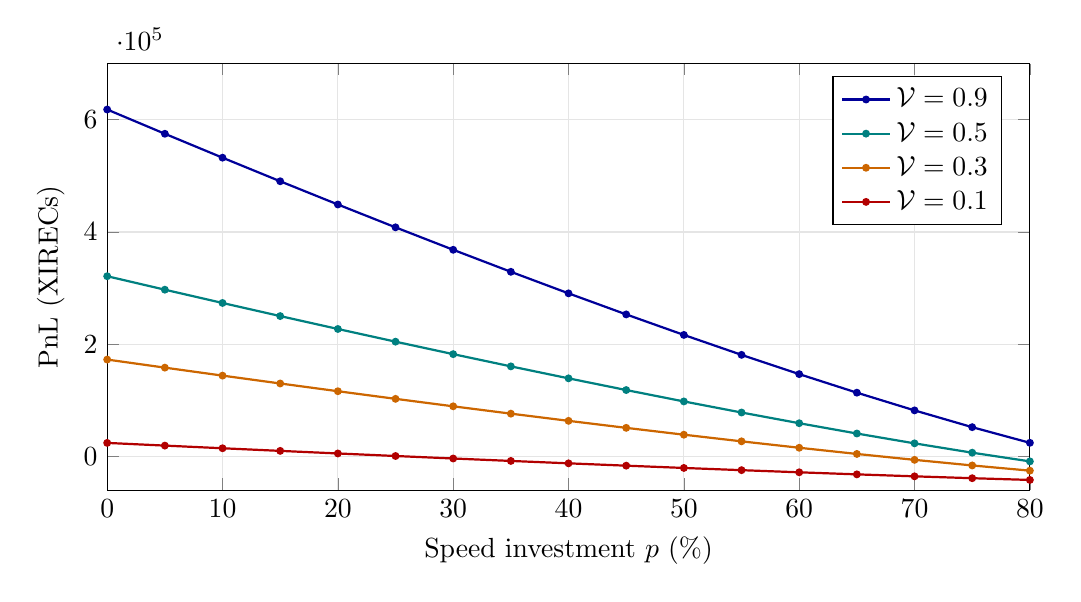
\begin{tikzpicture}
\begin{axis}[
  width=13.3cm, height=7cm,
  xlabel={Speed investment $p$ (\%)},
  ylabel={PnL (XIRECs)},
  xmin=0, xmax=80, ymin=-60000, ymax=700000,
  grid=both, grid style={gray!20},
  legend pos=north east,
  legend cell align=left,
  /pgf/number format/use comma
]
% Exact g(p) values from the FOC: PnL = K * g(p) * S - 50000, K=3033.507
\addplot[thick, blue!60!black, mark=*, mark size=1pt]
  coordinates {
    (0,618103)(5,574917)(10,532305)(15,490296)
    (20,448924)(25,408226)(30,368246)(35,329032)
    (40,290639)(45,253132)(50,216586)(55,181092)
    (60,146758)(65,113720)(70,82148)(75,52266)
    (80,24384)
  };
\addplot[thick, teal, mark=*, mark size=1pt]
  coordinates {
    (0,321168)(5,297176)(10,273503)(15,250164)
    (20,227180)(25,204570)(30,182359)(35,160573)
    (40,139244)(45,118407)(50,98104)(55,78385)
    (60,59310)(65,40955)(70,23415)(75,6815)
    (80,-8676)
  };
\addplot[thick, orange!80!black, mark=*, mark size=1pt]
  coordinates {
    (0,172701)(5,158306)(10,144102)(15,130099)
    (20,116308)(25,102742)(30,89415)(35,76344)
    (40,63546)(45,51044)(50,38862)(55,27031)
    (60,15586)(65,4573)(70,-5951)(75,-15911)
    (80,-25205)
  };
\addplot[thick, red!70!black, mark=*, mark size=1pt]
  coordinates {
    (0,24234)(5,19435)(10,14701)(15,10033)
    (20,5436)(25,914)(30,-3528)(35,-7885)
    (40,-12151)(45,-16319)(50,-20379)(55,-24323)
    (60,-28138)(65,-31809)(70,-35317)(75,-38637)
    (80,-41735)
  };
\legend{$\Sp=0.9$, $\Sp=0.5$, $\Sp=0.3$, $\Sp=0.1$}
\end{axis}
\end{tikzpicture}
\end{center}

Each curve is monotonically decreasing in~\(p\): \emph{for any fixed Speed
multiplier \(\Sp\), spending more on Speed strictly reduces PnL}. The benefit of
\(p>0\) is therefore entirely in its effect on the realised \(\Sp\) through
rank, as quantified by Eq.~\eqref{eq:thrFbe}.

\subsection{Break-even Speed multipliers}

Let \(\Sp_{\rm be}(p)\coloneqq 0.1\cdot g(0)/g(p)\) be the Speed multiplier at
which allocating \(p\) and hitting \(\Sp_{\rm be}\) yields exactly the PnL of
bidding \(0\) with \(\Sp=0.1\). Equivalently, \(F_{\rm be}(p)=(\Sp_{\rm be}-0.1)/0.8\)
is the fraction of the field one would need to beat. Exact values:

\begin{center}
\renewcommand{\arraystretch}{1.10}
\begin{tabular}{r r r c}
\toprule
\(p\) (\%) & \(\Sp_{\rm be}(p)\) & \(F_{\rm be}(p)\) & Interpretation \\
\midrule
5  & 0.1069 & 0.0086 & beat \(\ge 0.86\%\) of field \\
10 & 0.1147 & 0.0184 & beat \(\ge 1.84\%\) of field \\
20 & 0.1339 & 0.0424 & beat \(\ge 4.24\%\) of field \\
30 & 0.1597 & 0.0747 & beat \(\ge 7.47\%\) of field \\
50 & 0.2506 & 0.1883 & beat \(\ge 18.8\%\) of field \\
80 & 0.8982 & 0.9977 & \parbox{5.7cm}{\raggedright feasible only by attaining rank~1\\ (need to beat \(\ge 99.8\%\) of field)} \\
\bottomrule
\end{tabular}
\end{center}

The table above answers a \emph{different} (simpler) question than that of
Section~\ref{sec:atom}: here the baseline comparison is
\((r^\star(100),s^\star(100),0)\) with the unique-bottom multiplier \(\Sp=0.1\).
Under a realistic bottom atom, the comparison baseline is higher and the
threshold becomes correspondingly harder to meet---that is the content of
the last column of the table in Section~\ref{sec:atom}.

%============================================================
\section{Strategy Recommendations}\label{sec:recs}
%============================================================

\subsection{Benchmarks}
\begin{itemize}[leftmargin=*,itemsep=2pt]
  \item \textbf{Monopolist bound.} If there is only one player (or the player is
  guaranteed rank~\(1\)): \(p=0,\ r=23.14,\ s=76.86,\ \Sp=0.9\), giving
  \[
  \Pi_{\max}= K\cdot 0.9\cdot 244.71-50{,}000\;\approx\;\boxed{618{,}103\text{ XIRECs}}.
  \]
  \item \textbf{Equilibrium bound.} Symmetric Nash payoff
  \(\approx 24{,}234\) (Theorem~\ref{thm:mixedNE}).
  \item \textbf{Do-nothing.} \(\Pi=0\) with \(r=s=p=0\) (worst legal play).
\end{itemize}

\subsection{PnL of candidate allocations}

We use integer allocations near the FOC optimum for each \(p\). All values are
exact to the nearest XIREC:

\begin{center}
\renewcommand{\arraystretch}{1.10}
\begin{tabular}{l r r r r r}
\toprule
Allocation & \(\Sp=0.9\) & \(\Sp=0.7\) & \(\Sp=0.5\) & \(\Sp=0.3\) & \(\Sp=0.1\) \\
\midrule
\((23,77,0)\)  & \(618{,}097\) & \(469{,}631\) & \(321{,}165\) & \(172{,}699\) & \(\phantom{-0}24{,}233\) \\
\((21,69,10)\) & \(532{,}293\) & \(402{,}895\) & \(273{,}496\) & \(144{,}098\) & \(\phantom{-0}14{,}699\) \\
\((19,61,20)\) & \(448{,}908\) & \(338{,}039\) & \(227{,}171\) & \(116{,}303\) & \(\phantom{-00}5{,}434\) \\
\((17,53,30)\) & \(368{,}232\) & \(275{,}291\) & \(182{,}351\) & \(\phantom{0}89{,}411\) & \(-3{,}530\) \\
\bottomrule
\end{tabular}
\end{center}

\subsection{Conditional recommendation}

The correct recommendation depends on the expected distribution of opponent
bids, parameterised here by the mass \(\pi_0\) of players at \(p=0\) (and
therefore by \(\Sp_0\), the multiplier earned by the \(p=0\) block).

\begin{recbox}
\textbf{Default (robust)}: play \(\boxed{(r,s,p)=(23,77,0)}\).

\textbf{Hedged alternative}: play \(\boxed{(r,s,p)=(21,69,10)}\) only if you
believe the opponent CDF satisfies \(G(10^{-})-G(0^{-}) > \Delta G_\star\),
where \(\Delta G_\star\) is read from the table in Section~\ref{sec:atom}:
\begin{center}
\begin{tabular}{l c c c c}
\toprule
Estimated \(\pi_0\) (mass at \(0\)) & \(0\) & \(0.15\) & \(0.30\) & \(0.50\) \\
Implied \(\Sp_0\) at \(p=0\) (\(N\!\to\!\infty\)) & \(0.10\) & \(0.22\) & \(0.34\) & \(0.50\) \\
Required \(\Delta G_\star\) for \(p=10\) to dominate \(p=0\) & \(0.018\) & \(0.041\) & \(0.063\) & \(0.092\) \\
\bottomrule
\end{tabular}
\end{center}
\end{recbox}

\paragraph{Why not more Speed?} The required \(\Delta G_\star\) for \(p=20\)
is already \(\ge 0.07\) even against a lone-bottom baseline, and exceeds
\(0.14\) once \(\pi_0>0.3\); for \(p=30\) the number is \(0.25\) under similar
assumptions. These figures require the majority of the field to cluster below
\(20\) or \(30\)---unlikely in an environment where many players also attempt
speed-heavy allocations.

\paragraph{Cost of the hedge at best and worst.}
Relative to \((23,77,0)\), the allocation \((21,69,10)\) costs
\(618{,}103-532{,}293=85{,}810\) XIRECs if both attain \(\Sp=0.9\), and costs
\(24{,}233-14{,}699=9{,}534\) XIRECs if both attain \(\Sp=0.1\). The hedge is
worth taking only if the Speed-rank gain \(\Sp_{10}-\Sp_0\) compensates via the
mechanism of Eq.~\eqref{eq:thrFbe}.

\paragraph{When to prefer the purist \((23,77,0)\).} If you believe either (a)
a large fraction of the field will also bid \(p=0\), so the \(p=0\) tied block
already earns a healthy \(\Sp_0\); or (b) there is little mass in
\((0,10]\) because other players who move off~\(0\) go straight to
\(20\)--\(30\)---then \((23,77,0)\) strictly dominates the hedge. Our base-case
prior, consistent with historical manual-challenge distributions, places
\(\pi_0\in[0.15,0.35]\) and only \(\sim 5\%\) of players in \((0,10]\), in
which case \emph{the purist allocation has the higher expected value}.

%============================================================
\section{Verifying and Predicting the Speed Distribution}\label{sec:predict}
%============================================================

The entire quality of a final submission hinges on a prior over the opponent
distribution of~\(p\). This section lists concrete methods---ranked by
trustworthiness---to construct that prior.

\subsection{Historical calibration}
Previous Prosperity rounds (1--3) contained manual challenges with rank-based
pay-offs. Two robust stylised facts emerge from their post-round histograms:
\begin{enumerate}[leftmargin=*,itemsep=2pt]
  \item[(H1)] There is almost always a \textbf{large atom at the ``safe'' or
  ``obvious'' choice} (\(\sim\!25\)--\(40\%\) of the field).
  \item[(H2)] The remaining mass is bimodal: an ``equal-splitters'' bump (around
  \(p\approx 33\)) and a long right tail of aggressive bidders.
\end{enumerate}
Under (H1)+(H2), the mass in \((0,10]\) is typically small ($<10\%$), so
\(\Delta G\) rarely reaches the break-even thresholds of
Section~\ref{sec:atom} for \(\pi_0\in[0.25,0.4]\). This argues for the purist
\((23,77,0)\) as the base-case choice.

\subsection{Simulation under parametric priors}
Fix a mixture model for opponent behaviour, e.g.\
\[
p_{-i}\;\sim\;\pi_0\,\delta_0 + \pi_1\,\mathrm{Uniform}(0,15) + \pi_2\,\mathrm{Normal}(33,7) + \pi_3\,\mathrm{Uniform}(50,80),
\]
with weights \((\pi_0,\pi_1,\pi_2,\pi_3)\) summing to one. For each candidate
own-bid \(p\), Monte-Carlo a population of \(N\approx 3000\) opponents, compute
ranks per~\eqref{eq:speedlinear}, derive \(\Sp\), and evaluate~\(\Pi(p,\Sp)\).
Report mean, \(5\)th percentile, and \(95\)th percentile of PnL. Sweep \(p\) on
a grid of \(1\%\) increments to identify the \emph{robust} maximiser---i.e.\
the bid with the highest 5th-percentile PnL (CVaR rule).

\subsection{Bayesian update from community chatter}
Throughout each round, players discuss strategy on the official Discord.
Observed shifts in rhetoric (``everyone is going all-in on Speed'',
``Speed is a trap'') should be translated into updates on the mixture weights
\((\pi_0,\ldots,\pi_3)\). A disciplined protocol:
\begin{enumerate}[leftmargin=*,itemsep=2pt]
  \item At \(T=0\), set a prior from historical data (Section~7.1).
  \item Each hour, re-estimate \((\pi_0,\ldots,\pi_3)\) from a small sample of
  Discord messages classified by heuristic keywords.
  \item Recompute the robust maximiser and re-submit if it has moved by more
  than \(2\%\) in any pillar.
\end{enumerate}

\subsection{Post-round verification protocol}
After submission closes, leaderboard snapshots usually reveal enough
information to back out each player's realised Speed multiplier (from their
published PnL and their Research/Scale allocation, once visible). Compute:
\begin{itemize}[leftmargin=*,itemsep=2pt]
  \item empirical CDF \(\hat F(p)\) of opponent bids,
  \item mean Speed achieved by the \(p=0\) group,
  \item realised rent dissipation relative to the monopolist bound.
\end{itemize}
Compare with the equilibrium predictions of Theorem~\ref{thm:mixedNE} and
update your mixture model's priors for future rounds.

\subsection{A one-line sanity check}
Before submission, verify
\[
\R(r)\,\Sc(s)\cdot 0.1\;>\;50{,}000,
\]
i.e.\ that even with the worst Speed multiplier the net PnL is non-negative.
For \((23,77,0)\): \(\R(23)\Sc(77)\cdot 0.1 = K\cdot 244.71\cdot 0.1
=74{,}233>50{,}000\), margin \(\approx +24{,}233\). \checkmark For
\((21,69,10)\): \(K\cdot 213.29\cdot 0.1=64{,}699>50{,}000\), margin
\(\approx +14{,}699\). \checkmark

%============================================================
\section{Conclusions}
%============================================================

The Invest \& Expand challenge decomposes cleanly into (i)~a single-player
concave optimisation solvable in closed form via \(u(1+\ln u)=B+1\), and
(ii)~a rank auction whose symmetric Nash equilibrium dissipates \(\sim 96\%\) of
the monopolist surplus. The practical lever is that the field is \emph{not}
symmetric-Nash: it contains systematic over- and under-bidders, plus large
atoms at focal points. Whether a small Speed investment pays is decided by the
break-even condition
\(0.8\bigl(G(p^{-})-G(0^{-})\bigr)>\Sp_0\bigl(g(0)/g(p)-1\bigr)\), which for
\(p=10\) requires roughly \(\Delta G\ge 0.018\) against a lone-bottom baseline
and \(\Delta G\ge 0.063\) against a \(30\%\) bottom atom. Under our base-case
prior, not enough mass sits in \((0,10]\) to clear this bar, and the purist
allocation \((23,77,0)\) is the recommended submission; \((21,69,10)\) remains
a defensible hedge for priors with thin bottom atoms and non-trivial
\((0,10]\) mass. \emph{The final number that should be checked at submission
time is not an allocation but a belief about \(G\).}

\end{document}
